\documentclass{article}%
\usepackage[T1]{fontenc}%
\usepackage[utf8]{inputenc}%
\usepackage{lmodern}%
\usepackage{textcomp}%
\usepackage{lastpage}%
\usepackage{authblk}%
\usepackage{graphicx}%
%
\title{Infection by Streptococcus pyogenes Induces the Receptor Activator of NF{-}\_\_B Ligand Expression in Mouse Osteoblastic Cells}%
\author{John Lopez}%
\affil{Institute of Medicine, Chung Shan Medical University, No. 110, Section 1, Jianguo N. Road, Taichung 402, Taiwan}%
\date{01{-}01{-}2014}%
%
\begin{document}%
\normalsize%
\maketitle%
\section{Abstract}%
\label{sec:Abstract}%
STATEMENTS/COMMENTARY FROM UNIVERSITY OF SAN DIEGO\newline%
WASHINGTON D.C. {-} Researchers from the University of San Diego and University of South Carolina have successfully documented the involvement of a viral RNA{-}seq analysis tool among several samples derived from mice and flies.\newline%
The analysis technique, thought to be less sophisticated than the one used by Virat{-}seq, allows researchers to quickly identify small differences in DNA copies of circulating viral viral RNA and determine the synergies involved in developing viral proteins.\newline%
Readers may also read:\newline%
RNA{-}seq Analysis of Virat{-}seq Gossip\newline%
The critical physical properties of messenger RNA are important undergirding factors for generating proteins. The findings by the scientists detail an interaction between viral RNA{-}seq analysis and Virat{-}seq, which indicates that viral RNA{-}seq analysis provides an easy, sensitive way to identify significant biological characteristics of viral proteins.\newline%
Daniel Hudson, PhD, UCSD, Infectious Diseases Department\newline%
UNIVERSITY OF SAN DIEGO

%
\subsection{Image Analysis}%
\label{subsec:ImageAnalysis}%


\begin{figure}[h!]%
\centering%
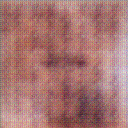
\includegraphics[width=150px]{500_fake_images/samples_5_33.png}%
\caption{A Black And White Photo Of A Black And White Cat}%
\end{figure}

%
\end{document}